% 原书PDF第76页4.5.2.2至第83页4.5.3之前。
\providecommand{\chFourAProj}{\bigl[I_{r_i}\otimes X(X^TX)^{-1}X^T\bigr]}
\providecommand{\chFourARisingDots}{\reflectbox{\ensuremath{\ddots}}}
\subsubsection{低秩表示诱导的因果网络}
假设有 $K$ 条通路或 $K$ 个簇，第 $k$ 条通路或簇含 $m_k$ 个基因。定义数据矩阵
\begin{equation}
\Upsilon=\begin{bmatrix}
y_{11}^1&\cdots&y_{1m_1}^1&y_{11}^2&\cdots&y_{1m_2}^2&\cdots&y_{11}^K&\cdots&y_{1m_K}^K\\
y_{21}^1&\cdots&y_{2m_1}^1&y_{21}^2&\cdots&y_{2m_2}^2&\cdots&y_{21}^K&\cdots&y_{2m_K}^K\\
\vdots&\ddots&\chFourARisingDots&\ddots&\chFourARisingDots&\ddots&\chFourARisingDots&\ddots&\chFourARisingDots&\vdots\\
y_{n1}^1&\cdots&y_{nm_1}^1&y_{n1}^2&\cdots&y_{nm_2}^2&\cdots&y_{n1}^K&\cdots&y_{nm_K}^K
\end{bmatrix}_{n\times M},
\tag{4.156}
\end{equation}
其中 $M=\sum_{i=1}^{K}m_i$。系数矩阵 $\Gamma$ 可分为对应于 $K$ 条通路或簇的 $K\times K$ 个子矩阵：
\begin{equation}
\Gamma=\begin{bmatrix}
\Gamma^{11}&\Gamma^{12}&\cdots&\Gamma^{1K}\\
\Gamma^{21}&\Gamma^{22}&\cdots&\Gamma^{2K}\\
\vdots&\vdots&\vdots&\vdots\\
\Gamma^{K1}&\Gamma^{K2}&\cdots&\Gamma^{KK}
\end{bmatrix}_{M\times M},
\tag{4.157}
\end{equation}
其中
\begin{equation}
\Gamma^{ij}=\begin{bmatrix}
\gamma_{11}^{ij}&\gamma_{12}^{ij}&\cdots&\gamma_{1m_j}^{ij}\\
\gamma_{21}^{ij}&\gamma_{22}^{ij}&\cdots&\gamma_{2m_j}^{ij}\\
\vdots&\vdots&\cdots&\vdots\\
\gamma_{m_i1}^{ij}&\gamma_{m_i2}^{ij}&\cdots&\gamma_{m_im_j}^{ij}
\end{bmatrix},\quad i,j=1,2,\ldots,K.
\tag{4.158}
\end{equation}
式 (4.150) 中表达数据矩阵 $\Upsilon^T\in\mathbb R^{M\times n}$ 的低秩表示为
\begin{equation}
\Upsilon^T=AZ+E,
\tag{4.159}
\end{equation}
其中
\begin{equation}
\begin{gathered}
A=\begin{bmatrix}A^1&0&\cdots&0\\0&A^2&\cdots&0\\\vdots&\vdots&\vdots&\vdots\\0&0&\cdots&A^K\end{bmatrix}_{M\times r},\\
A^k=\begin{bmatrix}
a_{11}^k&a_{12}^k&\cdots&a_{1r_k}^k\\
a_{21}^k&a_{22}^k&\cdots&a_{2r_k}^k\\
\vdots&\vdots&\vdots&\vdots\\
a_{m_k1}^k&a_{m_k2}^k&\cdots&a_{m_kr_k}^k
\end{bmatrix}_{m_k\times r_k},\quad k=1,\ldots,K,
\end{gathered}
\tag{4.160}
\end{equation}
\begin{equation}
\begin{gathered}
Z=\begin{bmatrix}Z^1\\Z^2\\\vdots\\Z^K\end{bmatrix}_{r\times n},\qquad
Z^k=\begin{bmatrix}
z_{11}^k&z_{12}^k&\cdots&z_{1n}^k\\
z_{21}^k&z_{22}^k&\cdots&z_{2n}^k\\
\vdots&\vdots&\vdots&\vdots\\
z_{r_k1}^k&z_{r_k2}^k&\cdots&z_{r_kn}^k
\end{bmatrix}_{r_k\times rn},\qquad r=\sum_{k=1}^{K}r_k.
\end{gathered}
\tag{4.161}
\end{equation}
令
\begin{equation}
G=Z^T=[(Z^1)^T\;(Z^2)^T\;\cdots\;(Z^K)^T]
=[G^1\;G^2\;\cdots\;G^K]_{n\times r},
\tag{4.162}
\end{equation}
其中
\[
G^k=\begin{bmatrix}
g_{11}^k&g_{12}^k&\cdots&g_{1r_k}^k\\
g_{21}^k&g_{22}^k&\cdots&g_{2r_k}^k\\
\vdots&\vdots&\vdots&\vdots\\
g_{n1}^k&g_{n2}^k&\cdots&g_{nr_k}^k
\end{bmatrix}_{n\times r_k}
=\begin{bmatrix}
z_{11}^k&z_{21}^k&\cdots&z_{r_k1}^k\\
z_{12}^k&z_{22}^k&\cdots&z_{r_k2}^k\\
\vdots&\vdots&\vdots&\vdots\\
z_{1n}^k&z_{2n}^k&\cdots&z_{r_kn}^k
\end{bmatrix}.
\]
令
\begin{equation}
\alpha=A^T\Gamma.
\tag{4.163}
\end{equation}
将式 (4.156) 与 (4.159) 代入式 (4.163)，得到
\begin{equation}
\begin{aligned}
\alpha&=\begin{bmatrix}
(A^1)^T\Gamma^{11}&(A^1)^T\Gamma^{12}&\cdots&(A^1)^T\Gamma^{1K}\\
(A^2)^T\Gamma^{21}&(A^2)^T\Gamma^{22}&\cdots&(A^2)^T\Gamma^{2K}\\
\vdots&\vdots&\vdots&\vdots\\
(A^K)^T\Gamma^{K1}&(A^K)^T\Gamma^{K2}&\cdots&(A^K)^T\Gamma^{KK}
\end{bmatrix}_{r\times M}\\
&=\begin{bmatrix}
\alpha^{11}&\alpha^{12}&\cdots&\alpha^{1K}\\
\alpha^{21}&\alpha^{22}&\cdots&\alpha^{2K}\\
\vdots&\vdots&\vdots&\vdots\\
\alpha^{K1}&\alpha^{K2}&\cdots&\alpha^{KK}
\end{bmatrix}_{r\times M},
\end{aligned}
\tag{4.164}
\end{equation}
其中
\begin{equation}
\alpha^{kj}=(A^k)^T\Gamma^{kj}
=\begin{bmatrix}
\alpha_{11}^{kj}&\alpha_{12}^{kj}&\cdots&\alpha_{1m_j}^{kj}\\
\alpha_{21}^{kj}&\alpha_{22}^{kj}&\cdots&\alpha_{2m_j}^{kj}\\
\vdots&\vdots&\vdots&\vdots\\
\alpha_{r_k1}^{kj}&\alpha_{r_k2}^{kj}&\cdots&\alpha_{r_km_j}^{kj}
\end{bmatrix}.
\tag{4.165}
\end{equation}
低秩表示诱导的线性结构方程模型可表述为
\begin{equation}
G\alpha+XB+E=0,
\tag{4.166}
\end{equation}
其中 $G$ 与 $\alpha$ 的定义同前，
\[
X=[X^1\;X^2\;\cdots\;X^L]
=\begin{bmatrix}x_{11}&x_{12}&\cdots&x_{1L}\\x_{21}&x_{22}&\cdots&x_{2L}\\\vdots&\vdots&\ddots&\vdots\\x_{n1}&x_{n2}&\cdots&x_{nL}\end{bmatrix},
\]
\[
B=[B^1\;B^2\;\cdots\;B^K],\qquad
B^i=\begin{bmatrix}
\beta_{11}^i&\beta_{12}^i&\cdots&\beta_{1r_i}^i\\
\beta_{21}^i&\beta_{22}^i&\cdots&\beta_{2r_i}^i\\
\vdots&\vdots&\vdots&\vdots\\
\beta_{L1}^i&\beta_{L2}^i&\cdots&\beta_{Lr_i}^i
\end{bmatrix},
\]
以及
\[
E=[E^1\;E^2\;\cdots\;E^K],\qquad
E^i=\begin{bmatrix}
e_{11}^i&e_{12}^i&\cdots&e_{1r_i}^i\\
e_{21}^i&e_{22}^i&\cdots&e_{2r_i}^i\\
\vdots&\vdots&\vdots&\vdots\\
e_{n1}^i&e_{n2}^i&\cdots&e_{nr_i}^i
\end{bmatrix}.
\]
它与经典标量线性结构方程模型的区别在于：经典模型的每个节点表示一个随机变量，而低秩表示诱导的模型中，每个节点表示随机变量向量。因此，节点 $i$ 对应的矩阵方程为
\begin{equation}
G\alpha^i+XB^i+E^i=0,
\tag{4.167}
\end{equation}
或
\[
\begin{aligned}
G^i={}&G^1\alpha^{1i}+\cdots+G^{i-1}\alpha^{i-1i}
+G^{i+1}\alpha^{i+1i}\\
&+\cdots G^K\alpha^{Ki}+XB^i+E^i,
\end{aligned}
\]
其中 $\alpha^{-i}$ 为所有其他节点指向节点 $i$ 的路径系数矩阵。$\alpha^{ji}$ 衡量从向量 $G^j$ 到 $G^i$，即节点 $j$ 到节点 $i$ 的因果关系强度；$\beta_l^i$ 为外生变量到内生变量的路径系数，衡量外生变量 $x_l$ 对低秩表示得分向量 $G^i$ 的因果效应。$\lVert\alpha^{ji}\rVert_{2,1}=0$ 与 $\lVert\beta_l^i\rVert_{2,1}=0$ 分别表示 $G^j$ 与 $x_l$ 对 $G^i$ 没有直接影响，通常从方程中省略。

令 $g^i=\operatorname{vec}(G^i)$ 为节点（通路）$i$ 基因表达低秩表示得分的 $nr_i$ 维向量；$e_i=\operatorname{vec}(E^i)$ 为对应的 $nr_i$ 维随机误差向量；$\delta_{ji}=\operatorname{vec}(\alpha^{ji})$（$j=1,\ldots,i-1,i+1,\ldots,K$）为节点 $j$ 到 $i$ 的 $r_jr_i$ 维路径系数向量。令
\[
\delta_i=[\delta_{1i}^T\;\cdots\;\delta_{i-1i}^T\;\delta_{i+1i}^T\;\cdots\;\delta_{Ki}^T]^T,
\]
其维数为 $J_i=(r_1+\cdots+r_{i-1}+r_{i+1}+\cdots+r_K)r_i$，表示所有其他节点指向节点 $i$ 的路径系数。再令
\[
b^i=\operatorname{vec}(B^i)=[(b_1^i)^T\;(b_2^i)^T\;\cdots\;(b_{r_i}^i)^T]^T,
\]
这是连接所有外生节点（基因型与环境节点）到节点 $i$ 的 $r_iL$ 维路径系数向量。附录4.D将证明，模型可写为
\begin{equation}
g^i=W_i\delta_i+H_ib^i+e_i,
\tag{4.168}
\end{equation}
其中 $e_i$ 为均值为零、协方差矩阵为 $\sigma_{ii}I_{r_in}$ 的 $r_in$ 维随机向量。式 (4.168) 两边左乘 $(I_{r_i}\otimes X)^T$，得到
\begin{equation}
(I_{r_i}\otimes X)^Tg^i
=(I_{r_i}\otimes X)^T(W_i\delta_i+H_ib^i)+(I_{r_i}\otimes X)^Te_i,
\tag{4.169}
\end{equation}
其中
\[
\Cov((I_{r_i}\otimes X)^Te_i,(I_{r_i}\otimes X)^Te_i)
=\sigma_{ii}(I_{r_i}\otimes X^TX).
\]
对式 (4.169) 应用加权最小二乘与 $l_2$ 范数惩罚，形成优化问题
\begin{equation}
\begin{aligned}
\min_{\delta_i,b^i}\quad&f(\delta_i,b^i)
+\lambda_1\left(\sum_{j=1}^{i-1}\lVert\delta_{ji}\rVert_2
+\sum_{j=i+1}^{K}\lVert\delta_{ji}\rVert_2\right)\\
&+\lambda_2\sum_{l=1}^{r_i}\lVert b_l^i\rVert_2,
\end{aligned}
\tag{4.170}
\end{equation}
其中
\[
\begin{aligned}
f(\delta_i,b^i)={}&\bigl[(I_{r_i}\otimes X)^Tg^i
-(I_{r_i}\otimes X)^T(W_i\delta_i+H_ib^i)\bigr]^T\\
&\quad\cdot(I_{r_i}\otimes X^TX)^{-1}\bigr)\\
&\quad*\bigl[(I_{r_i}\otimes X)^Tg^i
-(I_{r_i}\otimes X)^T(W_i\delta_i+H_ib^i)\bigr],
\end{aligned}
\]
\[
\lVert\alpha^{-i}\rVert_{2,1}=\sum_{j=1}^{i-1}\lVert\delta_{ji}\rVert_2
+\sum_{j=i+1}^{K}\lVert\delta_{ji}\rVert_2,\qquad
\lVert B^i\rVert_{2,1}=\sum_{i=1}^{r_i}\lVert b_l^i\rVert_2.
\]
矩阵 $M$ 的范数定义为 $\lVert M\rVert_{2,1}=\sum_j\lVert[M]_{:,j}\rVert_2$，其中 $[M]_{:,j}$ 为第 $j$ 个列向量。为将光滑优化 $\min f(\delta_i,b^i)$ 与非光滑项 $\lVert\alpha^{-i}\rVert_{2,1}$、$\lVert B^i\rVert_{2,1}$ 分离，引入约束 $\delta_{ji}-Z_j^1=0$ 与 $b_l^i-Z_l^2=0$，将问题 (4.170) 转化为
\begin{equation}
\begin{aligned}
\min_{\delta_i,b^i}\quad&f(\delta_i,b^i)
+\lambda_1\left(\sum_{j=1}^{i-1}\lVert Z_j^1\rVert_2
+\sum_{j=i+1}^{K}\lVert Z_j^1\rVert_2\right)\\
&+\lambda_2\sum_{l=1}^{r_i}\lVert Z_l^2\rVert_2,
\end{aligned}
\tag{4.171}
\end{equation}
约束为
\[
\begin{aligned}
\delta_{ji}-Z_j^1&=0,\quad j=1,\ldots,i-1,i+1,\ldots,K,\\
b_l^i-Z_l^2&=0,\quad l=1,\ldots,r_i.
\end{aligned}
\]
附录4.B证明，该问题可用 ADMM 求解，算法概括为结论4.7。

\par\medskip\Needspace{6\baselineskip}
\noindent\textbf{结论4.7：求解低秩表示诱导结构方程模型（LRRISEM）的 ADMM 算法}\par
对 $i=1,\ldots,K$，执行下列步骤。

\noindent\textbf{步骤1：初始化。}
\[
u^0:=0,\qquad v^0:=0,
\]
\[
\begin{aligned}
\delta_i^{(0)}={}&\left\{W_i^T\chFourAProj W_i+\rho_1I\right\}^{-1}\\
&\qquad\cdot W_i^T\chFourAProj g^i,
\end{aligned}
\]
\[
\begin{aligned}
(b^i)^{(0)}={}&\left\{H_i^T\chFourAProj H_i+\rho_2I\right\}^{-1}\\
&\qquad\cdot H_i^T\chFourAProj g^i,
\end{aligned}
\]
\[
(Z_j^1)^{(0)}=\frac{(\lVert\delta_{ji}^{(0)}\rVert_2-\lambda_1/\rho_1)_+}{\lVert\delta_{ji}^{(0)}\rVert_2}\delta_{ji}^{(0)},
\quad j=1,\ldots,i-1,i+1,\ldots,K,
\]
\[
(Z_l^2)^{(0)}=\frac{(\lVert(b_l^i)^{(0)}\rVert_2-\lambda_2/\rho_2)_+}{\lVert(b_l^i)^{(0)}\rVert_2}(b_l^i)^{(0)},
\quad l=1,\ldots,r_i.
\]
执行步骤2、3、4直到收敛。

\noindent\textbf{步骤2：}
\[
\begin{aligned}
\delta_i^{(k+1)}={}&\left\{W_i^T\chFourAProj W_i+\rho_1I\right\}^{-1}\\
&\quad\cdot\Bigl\{W_i^T\chFourAProj g^i+\rho_1((Z^1)^{(k)}-u^{(k)}\Bigr\},
\end{aligned}
\]
\[
\begin{aligned}
(b^i)^{k+1}={}&\left\{H_i^T\chFourAProj H_i+\rho_2I\right\}^{-1}\\
&\quad\cdot\Bigl\{H_i^T\chFourAProj g^i+\rho_2((Z^2)^{(k)}-v^{(k)}\Bigr\}.
\end{aligned}
\]
\noindent\textbf{步骤3：}
\[
\begin{aligned}
(Z_j^1)^{(k+1)}&=\frac{(\lVert\delta_{ji}^{(k+1)}+u_j^{(k)}\rVert_2-\lambda_1/\rho_1)_+}
{\lVert\delta_{ji}^{(k+1)}+u_j^{(k)}\rVert_2}
(\delta_{ji}^{(k+1)}+u_j^{(k)}),\\
&\hspace{22mm}j=1,\ldots,i-1,i+1,\ldots,K,
\end{aligned}
\]
\[
(Z_l^2)^{(k+1)}=\frac{(\lVert(b_l^i)^{(k+1)}+v_l^{(k)}\rVert_2-\lambda_2/\rho_2)_+}
{\lVert(b_l^i)^{(k+1)}+v_l^{(k)}\rVert_2}
((b_l^i)^{(k+1)}+v_l^{(k)}),\quad l=1,\ldots,r_i.
\]
\noindent\textbf{步骤4：}
\[
\begin{aligned}
u_j^{(k+1)}&\mathrel{:==}u_j^{(k+1)}+(\delta_{ji}^{(k+1)}-(Z_j^1)^{(k+1)}),\\
&\hspace{22mm}j=1,\ldots,i-1,i+1,\ldots,K,\\
v_l^{(k+1)}&\mathrel{:==}v_l^{(k)}+((b_l^i)^{(k+1)}-(Z_l^2)^{(k+1)}),\quad l=1,\ldots,r_i.
\end{aligned}
\]

\begin{bookexample}{4.8}
将低秩表示诱导结构方程模型与整数规划结合的算法（LRRISEMIG），应用于447个样本中24条信号转导通路、1728个基因的 RNA-seq 数据。估计的调控网络见图4.22。LRRISEMIG 估计出50条有向边，其中25条与 KEGG 通路数据库中的路径方向一致。KEGG 数据库共含69条路径。

将 LRRISEMIG 与贝叶斯网络及随机网络比较，进行10000次模拟，计算检出有向边总数、正确识别的有向边数与错误识别边数的均值。检出功效与假阳性率定义为
\[
\text{检出功效}=\frac{\text{检出的真实路径数}}{\text{估计的边数}},\qquad
\text{假阳性率}=\frac{\text{估计的错误边数}}{\text{标记的边数}}.
\]
比较中使用 R 包 bnlearn。它实现了针对离散、高斯和条件高斯网络的多种结构学习算法，包括基于约束的 GS、IAMB、Inter-IAMB、Fast-IAMB、MMPC、Hiton-PC，成对方法 ARACNE 与 Chow-Liu，基于评分的爬山法与 Tabu 搜索，以及混合方法 MMHC 与 RSMAX2，并提供多种评分函数和条件独立检验（Scutari 2017）。结果见表4.12。LRRISEMIG 的表现远好于随机构建的网络，说明其推断的调控网络具有生物学意义。与新近发布的贝叶斯网络推断包 bnlearn 相比，LRRISEMIG 的检出功效较高，假阳性率较低。
\end{bookexample}
\begin{figure}[p]
\centering
\begin{tikzpicture}[x=1cm,y=1cm]
\node[anchor=south west,inner sep=0] at (0,0) {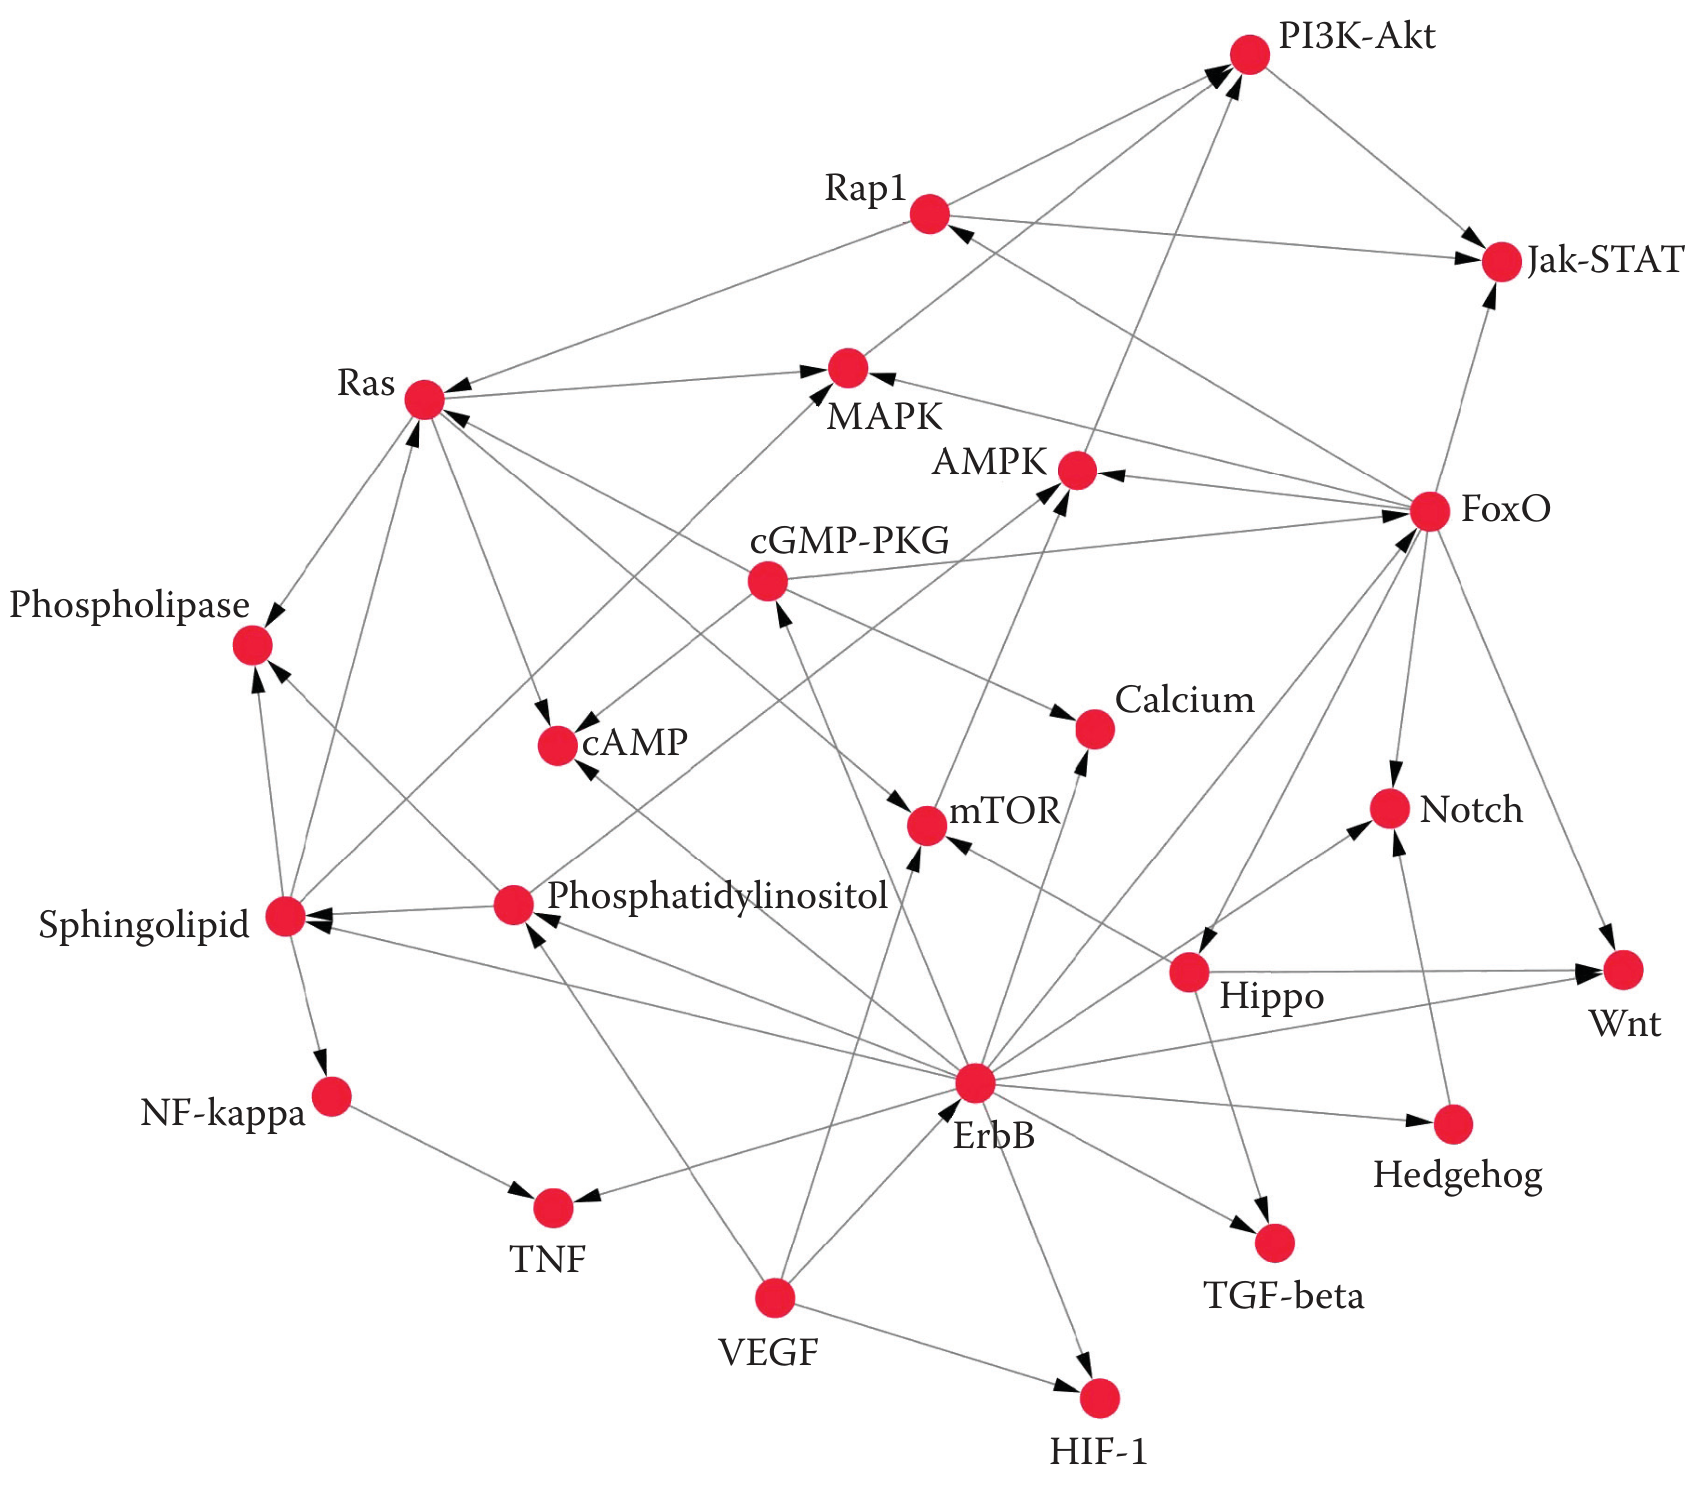
\includegraphics[width=13.5cm]{figures/ch04a_fig22_data.png}};
\fill[white] (0.0438,6.9083) rectangle (2.0215,7.2778);
\node[inner sep=0pt,fill=white,rotate=0,font=\fontsize{8}{8}\selectfont] at (1.0326,7.0930) {磷脂酶};
\fill[white] (0.2795,4.3539) rectangle (2.0232,4.7234);
\node[inner sep=0pt,fill=white,rotate=0,font=\fontsize{8}{8}\selectfont] at (1.1514,4.5387) {鞘脂};
\fill[white] (8.8776,6.1496) rectangle (10.0530,6.5192);
\node[inner sep=0pt,fill=white,rotate=0,font=\fontsize{8}{8}\selectfont] at (9.4653,6.3344) {钙};
\fill[white] (4.3388,4.5856) rectangle (7.1204,4.9551);
\node[inner sep=0pt,fill=white,rotate=0,font=\fontsize{8}{8}\selectfont] at (5.7296,4.7703) {磷脂酰肌醇};
\end{tikzpicture}
\origfig{22}{结合整数规划的低秩表示诱导结构方程模型估计的24条信号转导通路调控网络。}
\label{fig:ch04a-22}
\end{figure}

\begin{table}[htbp]
\centering\small
\origtable{12}{检出功效与假阳性率}
\begin{tabular}{lrrrrr}
\toprule
&\shortstack{检出\\边数}&\shortstack{与 KEGG\\一致的边数}&假阳性&检出功效&假阳性率\\
\midrule
LRRISEMIG&58&29&29&50.00\%&42.00\%\\
bnlearn&58&25&33&43.10\%&47.80\%\\
随机网络&58&15&43&25.90\%&62.30\%\\
\bottomrule
\end{tabular}
\end{table}

\FloatBarrier
